\documentclass[10pt, oneside, letterpaper]{article}
\usepackage[margin=1in]{geometry}
\usepackage[english]{babel}
\usepackage[utf8]{inputenc}
\usepackage{xcolor}
\definecolor{mygreen}{rgb}{0,0.6,0}
\definecolor{mygray}{rgb}{0.5,0.5,0.5}
\definecolor{mymauve}{rgb}{0.58,0,0.82}
\usepackage{listings}
\lstset{
  backgroundcolor=\color{white}, % choose the background color
  basicstyle=\footnotesize\ttfamily, % size of fonts used for the code
  breaklines=true, % automatic line breaking only at whitespace
  frame=single, % add a frame
  captionpos=b, % sets the caption-position to bottom
  commentstyle=\color{mygreen}, % comment style
  escapeinside={\%*}{*)}, % if you want to add LaTeX within your code
  keywordstyle=\color{blue}, % keyword style
  stringstyle=\color{mymauve}, % string literal style
}
\usepackage{enumitem}
\usepackage{blindtext}
\usepackage{datetime2}
\usepackage{fancyhdr}
\usepackage{amsmath}
  \newcommand{\angstrom}{\textup{\AA}} % for units of angstrom
\usepackage{arydshln} % dash line package for matrices
\usepackage{mathtools} % for things like \Aboxed
\usepackage{float}
\usepackage{pgf}
\usepackage{enumitem} % to easily change style of counters in item lists
\usepackage{xurl} % to easily insert URLs in the LaTeX source
\usepackage{braket} % for bra-ket notation
\usepackage{bm} % for bold vector variables
\usepackage{cases} % for piecewise definitions
\usepackage[makeroom]{cancel} % for crossing out terms
\usepackage{graphicx} % for \scalebox
  \newcommand\scalemath[2]{\scalebox{#1}{\mbox{\ensuremath{\displaystyle #2}}}}

\setcounter{MaxMatrixCols}{32} % increase the maximum number of matrix columns

\title{Assignment 3}
\author{Calculating Electronic Structures of the \\ Helium atom and Hydrogen Molecule using \\Hartree-Fock and Roothaan Equations}
\date{Due: 2022/03/04}

\pagestyle{fancy}
\setlength{\headheight}{23pt}
\setlength{\parskip}{1em}
\fancyhf{}
\chead{Assignment 3}
\rhead{Michel Kakulphimp \\ Student \#63542880}
\lhead{ELEC542 \\ UBC MEng}
\cfoot{\thepage}

\begin{document}
\maketitle
\thispagestyle{fancy}

\section{Directions}

This is a direct follow-up to assignment 2. We are interested in solving the same two systems (hydrogen molecule and helium atom) as in that assignment and comparing the results with what we obtained there.

In this assignment, use the Roothaan equation. As basis functions, use two s-type, normalized Gaussian functions (with different values of $\alpha$) centered on each atom. Note that you can choose whatever values of $\alpha$ you find most suitable for the two Gaussian functions on each atom. Play around with a few different $\alpha$ values to see which ones give you the most reasonable answers. If you are ambitious, include additional basis functions.

\begin{enumerate}[label=(\alph*)]
  \item (4 points) Describe your approach and show the steps of your derivation all the way to obtaining the matrix equation.
  \item (4 points) Write a computer code to implement what you built in part a.
  \item (4 points) Plot several molecular orbitals and give their associated energies for the helium atom. Also calculate the total energy of the system. Discuss your results.
  \item (4 points) Plot several molecular orbitals and give their associated energies for the hydrogen molecule. Also calculate the total energy of the system (not including the nucleus-nucleus interaction). Discuss your results.
  \item (4 points) Compare your results of both the above exercise and what you obtained in assignment 2 together and also with values available from the literature, and what you obtain using a commercial program such as Gaussian (run through ABACUS, for example).
\end{enumerate}

\section{Derivation of Solution}

As with the previous assignment, since both subjects for this assignment have an even number of electrons that close shells, we can use the restricted Hartree-Fock equation for closed shell systems to numerically calculate the resulting orbitals. The equation is as follows:

\begin{align*}
  \hat{F}(\vec{r})\psi_n(\vec{r}) &= \epsilon_n\psi_n(\vec{r})
\end{align*}

Where $\hat{F}(\vec{r})$ is the Fock operator which is defined as follows:

\begin{align*}
  \hat{F}(\vec{r}) &= \hat{H}_{core}(\vec{r}) + \sum_{n=1}^{N/2}\left[2J_n(\vec{r}) - K_n(\vec{r})\right]\\
\end{align*}

In the previous assignment, the wave equation $\psi_n(\vec{r})$ was obtained by discretizing the solution of the wave equation into a three-dimensional grid partition of size $N \times N \times N$ where each dimension was partitioned into $N$ elements. The Hartree-Fock equation was manipulated to create a matrix eigenvector/eigenvalue problem out of the wave equation to be solved iteratively by a computer program over this space. The largest computational load in the previous assignment's program turned out to be the integration that needed to be performed for every iteration. The exchange term has an integral to calculate over the $N \times N \times N$ space of the matrix. This meant that for every element in the $N \times N \times N$ space, the integration had to be performed over a space of $N \times N \times N$. This integral alone resulted in $N^6$ calculations during every iteration of the Hartree-Fock algorithm. Multiprocessing helped alleviate some of this load by spreading it across multple processing units, but the problem was still very taxing to a modern computer with a modest number of spatial partitions.

\subsection{Introducing Basis through the Roothaan Equations}

This assignment aims to simplify the Hartree-Fock procedure by introducing the concept of basis functions. The following derivations are presented in Szabo and Ostlund (referenced at the end of this assignment) and are summarized in the following paragraphs. Known as the Roothaan equations, the Hartree-Fock equation is augmented by using a combination of non-orthonormal spatial basis functions. The Hartree-Fock procedure is now modified to converge on the coefficients of these basis functions which linearly combine to approximate the electron orbitals. These functions are chosen very carefully to approximate the orbital that the electrons should exist in, which allows a small combination of them to simulate a real system with high accuracy. Likely more accurate and more stable than what was implemented in the previous assignment. Since there are only a few coefficients to solve for in this basis set of functions, the Hartree-Fock procedure is greatly simplified when put into a matrix eigenvector/eigenvalue problem. The basis functions can be described as follows:

\begin{align*}
  \psi_n(\vec{r}) &= \sum_{\mu = 1}^K C_{\mu n}\phi_\mu(\vec{r}) \qquad n = 1, 2, ... , K
\end{align*}

A complete set of functions $\phi_\mu$ could exactly represent a system; however, for computational practicality much less can be used, as is evident by this assignment only asking for two or more of these functions. Specifically, normalized gaussian functions are to be used in this assignment. When combined, two or more gaussian functions can better approximate the shape of an atomic orbital as a single gaussian function alone does not match the shape of an atomic orbital very well. A real orbital function will have a pointed asymptotic shape in the middle where the nucleus is present, wheras a gaussian function has a rounded shape at its maximum. By adding a combination of gaussian functions together, the pointed shape is better approximated. An advantage of using a combination of gaussian functions is that they are easily integrated. Since integration is a common operation in Hartree-Fock, this lends well to a rapid calculations towards a convergence.

By substituting the linear combination of functions of $\phi_\mu$ in the place of $\psi_n$ in the Hartree-Fock equation, we obtain the following:

\begin{align*}
  \hat{F}(\vec{r})\sum_{\mu = 1}^K C_{\mu n}\phi_\mu(\vec{r}) &= \epsilon_n\sum_{\mu = 1}^K C_{\mu n}\phi_\mu(\vec{r})
\end{align*}

We can then multiply both sides by $\phi_v^\ast(\vec{r})$ and integrate to obtain the following result:

\begin{align*}
  \sum_{\mu = 1}^K C_{\mu n} \int_{-\infty}^{\infty} \phi_v^\ast(\vec{r}) \hat{F}(\vec{r}) \phi_\mu(\vec{r})d\vec{r} &= \epsilon_n\sum_{\mu = 1}^K C_{\mu n}\int_{-\infty}^{\infty}\phi_v^\ast(\vec{r})\phi_\mu(\vec{r})d\vec{r}
\end{align*}

This allows the Hartree-Fock equation to be turned into a matrix equation containing the overlap matrix $\bm{S}$ containing $K \times K$ elements $S_{v\mu}$:

\begin{align*}
S_{v\mu} &= \int_{-\infty}^{\infty}\phi_v^\ast(\vec{r})\phi_\mu(\vec{r})d\vec{r}
\end{align*}

and the Fock matrix $\bm{F}$ containing $K \times K$ elements $F_{v\mu}$:

\begin{align*}
F_{v\mu} &= \int_{-\infty}^{\infty} \phi_v^\ast(\vec{r}) \hat{F}(\vec{r}) \phi_\mu(\vec{r})d\vec{r}
\end{align*}

Bringing these back into the Hartree-Fock equation, we obtain the following equation, known as the Roothan equations:

\begin{align*}
\sum_{\mu = 1}^K F_{v\mu} C_{\mu n} &= \epsilon_n\sum_{\mu = 1}^K S_{v\mu} C_{\mu n}
\end{align*}

or more concisely:

\begin{align*}
\bm{F}\bm{C} &= \bm{S}\bm{C}\bm{\epsilon}
\end{align*}

The matrix $\bm{C}$ is a $K \times K$ square matrix of the expansion coefficients $C_{\mu n}$:

\begin{align*}
\bm{C} =
\begin{bmatrix}
 C_{11} & C_{12} & \hdots & C_{1K}\\
 C_{21} & C_{22} & \hdots & C_{2K}\\
 \vdots & \vdots &        & \vdots \\
 C_{K1} & C_{K2} & \hdots & C_{KK}\\
\end{bmatrix}
\end{align*}

and $\bm{\epsilon}$ is a diagonal matrix of the orbital energies $\epsilon_n$:

\begin{align*}
\bm{\epsilon} =
\begin{bmatrix}
 \epsilon_1 &            &        & \\
            & \epsilon_2 &        & \\
            &            & \ddots & \\
            &            &        & \epsilon_K\\
\end{bmatrix}
\end{align*}

\subsection{Charge Density Matrix}

In order to calculate the Fock matrix $\bm{F}$, we have to introduce the concept of a charge density matrix. This matrix describes the probability distribution of finding an electron in a given space described by the wave function $\psi_n(\vec{r})$. In a closed-shell system described by a single wave function occupied by two electrons (as in this assignment), the total charge density $\rho(\vec{r})$ is equal to:

\begin{align*}
\rho(\vec{r}) &= 2 \sum_{n}^{N/2}\left|\psi_n(\vec{r})\right|^2
\end{align*}

We can then substitue the basis function expansion performed above to derive what is known as the density matrix $\bm{P}$:

\begin{align*}
\rho(\vec{r}) &= 2 \sum_{n}^{N/2}\psi_n^\ast(\vec{r})\psi_n(\vec{r}) \\
\rho(\vec{r}) &= 2 \sum_{n}^{N/2}\sum_{v = 1}^K C_{v n}^\ast\phi_v^\ast(\vec{r})\sum_{\mu = 1}^K C_{\mu n}\phi_\mu(\vec{r}) \\
\rho(\vec{r}) &= \sum_{v = 1}^K\sum_{\mu = 1}^K \left[ 2 \sum_{n}^{N/2} C_{v n}^\ast C_{\mu n} \right] \phi_v^\ast(\vec{r}) \phi_\mu(\vec{r}) \\
\rho(\vec{r}) &= \sum_{v = 1}^K\sum_{\mu = 1}^K P_{v\mu} \phi_v^\ast(\vec{r})\phi_\mu(\vec{r}) \\
P_{v\mu} &= 2 \sum_{n}^{N/2} C_{v n}^\ast C_{\mu n}
\end{align*}

The density matrix is composed of the coefficients of the basis functions, and it describes the charge density $\rho(\vec{r})$ for the electrons in the system.

Now we have all the pieces to expand the Fock operator into its new basis function matrix form:

\begin{align*}
  F_{v\mu} &= \int_{-\infty}^{\infty} \phi_v^\ast(\vec{r}) \hat{F}(\vec{r}) \phi_\mu(\vec{r})d\vec{r} \\
  F_{v\mu} &= \int_{-\infty}^{\infty} \phi_v^\ast(\vec{r}) \hat{H}(\vec{r}) \phi_\mu(\vec{r})d\vec{r} + \sum_{n=1}^{N/2} \int_{-\infty}^{\infty} \phi_v^\ast(\vec{r}) \left[2J_n(\vec{r}) - K_n(\vec{r})\right] \phi_\mu(\vec{r})d\vec{r} \\
  F_{v\mu} &= H_{v\mu}^{core} + \sum_{n=1}^{N/2} 2(v\mu|aa) - (va|\mu a)
\end{align*}

The core Hamiltonian matrix element $H_{v\mu}^{core}$ can be further expanded into the kinetic energy integrals $T_{v\mu}$ and nuclear attraction integrals $V_{v\mu}$:

\begin{align*}
  T_{v\mu} &= \int_{-\infty}^{\infty} \phi_v^\ast(\vec{r}) \left[ -\frac{1}{2}\nabla^2 \right] \phi_\mu(\vec{r})d\vec{r} \\
  V_{v\mu} &= \int_{-\infty}^{\infty} \phi_v^\ast(\vec{r}) \left[ -\sum_{A=1}^{M}\frac{Z_A}{\vec{r} - \vec{R}_A} \right] \phi_\mu(\vec{r})d\vec{r} \\
  H_{v\mu}^{core} &= T_{v\mu} + V_{v\mu}
\end{align*}

Interesting to note here is that the Hamiltonian matrix does not depend on the coefficients, which are the elements being iteratively solved in the algorithm. Therefore, the Hamiltonian matrix only needs to be evaluated once during the process. This is unlike the previous assignment, where the Hamiltonian needed to be evaluated at every iteration.

The last piece of the puzzle is to introduce the linear expansion into the two-electron integral using the work derived above for the density matrix $\bm{P}$:

\begin{align*}
  F_{v\mu} &= H_{v\mu}^{core} + \sum_{n=1}^{N/2} \sum_{\lambda = 1}^K\sum_{\sigma = 1}^K C_{\lambda n}^\ast C_{\sigma n} \left[ 2(v\mu|\sigma\lambda) - (v\lambda|\sigma\mu) \right] \\
  P_{\lambda\sigma} &= 2 \sum_{n}^{N/2} C_{\lambda n}^\ast C_{\sigma n} \\
  F_{v\mu} &= H_{v\mu}^{core} + \sum_{\lambda = 1}^K\sum_{\sigma = 1}^K P_{\lambda\sigma} \left[ (v\mu|\sigma\lambda) - \frac{1}{2}(v\lambda|\sigma\mu) \right] \\
  F_{v\mu} &= H_{v\mu}^{core} + G_{v\mu}
\end{align*}

The two-electron intergrals expand as follows:

\begin{align*}
  (v\mu|\sigma\lambda) &= \int_{-\infty}^{\infty}\int_{-\infty}^{\infty}  \phi_v^\ast(\vec{r}_1)\phi_\mu(\vec{r}_1) \frac{1}{\|\vec{r}_{12}\|}  \phi_\sigma^\ast(\vec{r}_2)\phi_\lambda(\vec{r}_2)  d\vec{r}_1d\vec{r}_2
\end{align*}

For every iteration of the Hartree-Fock algorithm, the matrix $\bm{G}$ will need to be recalculated which is reliant on the density matrix $\bm{P}$.

\subsection{Orthogonalization of the Basis}

In order to solve an eigenvalue problem on every iteration, it will be necessary to reconfigure the matrix Fock equation from:

\begin{align*}
\bm{F}\bm{C} &= \bm{S}\bm{C}\bm{\epsilon}
\end{align*}

to:

\begin{align*}
\bm{F}'\bm{C}' &= \bm{C}'\bm{\epsilon}
\end{align*}

Which is a form where the modified Fock matrix $\bm{F}'$ can be diagonalized to solve for $\bm{C}'$ which in turn is converted back into $\bm{C}$. In this modified equation, the overlap matrix $\bm{S}$ disappears as a transformation is applied to orthonormalize the basis functions. Note that the overlap matrix $\bm{S}$ is present because the basis functions chosen are not normally orthonormal.

A transformation matrix $\bm{X}$ needs to be found to satisfy the following condition:

\begin{align*}
\bm{X}^\dagger\bm{S}\bm{X} &= 1
\end{align*}

This assignment will using symmetric orthogonolization, which uses the inverse square root of $\bm{S}$ as $\bm{X}$:

\begin{align*}
\bm{X} &= \bm{S}^{-\frac{1}{2}}
\end{align*}

The expansion coefficient matrix $\bm{C}$ can then be transformed to and from its modified state using $\bm{X}$ as follows:

\begin{align*}
\bm{C}' &= \bm{X}^{-1}\bm{C} & \bm{C} &= \bm{X}\bm{C}'
\end{align*}

Similarly, the modified Fock matrix $\bm{F}'$ can be obtained as follows:

\begin{align*}
\bm{F}' &= \bm{X}^\dagger\bm{F}\bm{X}
\end{align*}

\subsection{Choosing the Basis}

For this assignment, the STO-1G basis sets will be used for the basis functions. STO-1G are Gaussian approximations of the more realistic Slater functions for orbitals (hence the namesake Slater-Type Orbital: STO) \cite{chem-libretext-gaussian-basis-sets}. These basis sets represent a 1s atomic orbital approximated by a single Gaussian function each and have the following generic form:

\begin{align*}
\phi &= ae^{-b\vec{r}^2}
\end{align*}

Tuned STO-1G basis functions were found in \cite[p.~214]{errol-comp-chem-text}\cite{hartree-fock-in-100-lines} for both the 1s orbital of the Hydrogen atom as well as the Helium atom with values for $a$ and $b$ as follows:

\begin{align*}
\phi_{H} &= 0.3696e^{-0.4166\left|\vec{r} - \vec{R}\right|^2} \\
\phi_{He} &= 0.5881e^{-0.7739\left|\vec{r} - \vec{R}\right|^2}
\end{align*}

For the Helium atom, two of the Helium 1s orbital STO-1G basis functions will be centered on the nucleus, which exists at the origin of the problem. For the Hydrogen molecule, two of the the Hydrogen 1s orbital STO-1G basis functions will be center on each nucleus, for a total of four basis functions. As calculated in the previous assignment, the distance between the two Hydrogen nuclei is $\frac{0.74 \times 0.1\times10^{-9}}{5.29177210903\times10^{-11}} = 1.39839733222307$ atomic units of length. The Hydrogen molecule nuclei will be placed on the $x$ axis.

\subsection{Precalculating the Integrals}

An advantage of using basis functions is that many of the integrals required for the resulting matrices can be pre-computed as they do not alter between iterations. For the one-electron integrals, one must calculate the kinetic energy integral for every entry in the kinetic energy matrix and the potential energy integral for the potential energy matrix. These two matrices make up the core Hamiltonian matrix which is composed of one-electron integrals. Similarly, one must calculate the two-electron integrals, however this piece is more complicated and more computationally involved. The result of these two-electron integrals will make up the $\bm{G}$ matrix mentioned previously, which consists of the density matrix $\bm{P}$ multiplied by the Coulomb repulsion two-electron integral and the exchange operator two-electron integral. Only the density matrix will be modified, so the two-electron integrals that the density matrix elements will be multiplying can be precomputed.

In order to ease the burden of integrating the two-electron integrals, they will be simplified by invoking the Gaussian product rule since Gaussian functions are used as the basis functions. This transforms the integrand from four centers ($\bm{A}$, $\bm{B}$, $\bm{C}$, $\bm{D}$) to two ($\bm{P}$, $\bm{Q}$). The integral is further simplified by replacing the factors of the resulting integrand with their Fourier transforms, which eventually collapses into a single integration. The full derivation can be found in \cite[p.~153-155,157]{molecular-integrals-over-gaussian-basis-functions}. This will simplify the two-electron integral to the following equivalent:

\begin{align*}
  (v\mu|\sigma\lambda) &= \int_{-\infty}^{\infty}\int_{-\infty}^{\infty}  \phi_v^\ast(\vec{r}_1)\phi_\mu(\vec{r}_1) \frac{1}{\|\vec{r}_{12}\|}  \phi_\sigma^\ast(\vec{r}_2)\phi_\lambda(\vec{r}_2)  d\vec{r}_1d\vec{r}_2
\end{align*}

\subsection{Calculating the Total Energy}

The total energy of the system can be obtained by 

\subsection{Final Recipe}

We now have all of the background required to implement our solution. The following steps outline what is required for this simulation to run:

\begin{enumerate}
    \item Prepare $K \times K$ matrices where $K$ corresponds to the number of basis functions
    \item Pre-calculate one and two-electron integrals using the specified basis set chosen
      \begin{itemize}
        \item Overlap matrix $\bm{S}$ containing one electron integrals $S_{v\mu}$
        \item Kinetic $\bm{T}$ energy matrix one electron integrals $T_{v\mu}$
        \item Nuclear attraction $\bm{V}$ matrix one electron integrals $V_{v\mu}$
        \item $\bm{G}$ matrix Coulomb repulsion and exchange two-electron integrals
      \end{itemize}
    \item Obtain the transformation matrix $\bm{X}$ by through the inverse square root of $\bm{S}$: $\bm{X} = \bm{S}^{-\frac{1}{2}}$
    \item Calculate the $\bm{G}$ matrix using the current density matrix $\bm{P}$ (zero on the first iteration) and the two-electron integrals
    \item Calculate the $\bm{F}$ Fock matrix using $\bm{T} + \bm{V} + \bm{G}$
    \item Apply the transformation matrix $\bm{X}$ to obtain the orthonormalized Fock matrix $\bm{F}' = \bm{X}^\dagger\bm{F}\bm{X}$:
    \item Diagonalize the orthonormalized Fock matrix $\bm{F}'$ to obtain the orthonormalized coefficient matrix $\bm{C}'$
    \item Convert the orthonormalized coefficient matrix $\bm{C}'$ to the regular coefficient matrix $\bm{C}$: $\bm{C} = \bm{X}\bm{C}'$
    \item Extract the coefficients from $\bm{C}$ to obtain a new version of the $\bm{P}$ matrix
    \item Compare this new density matrix $\bm{P}$ with the one we started with, if the difference between the two is not within a specified threshold, repeat the process from 4. If the difference between both $\bm{P}$ is within the threshold, the algorithm is complete.

\end{enumerate}

\newpage
\section{Program Implementation}

Precalculating the integrals will be performed by the program on startup and saved as comma-separated-value (CSV) file for easy lookup. Subsequent runs will load this data file and use the values and skip this step.

\newpage
\section{Results}

\begin{figure}[H]
  \begin{center}
    % 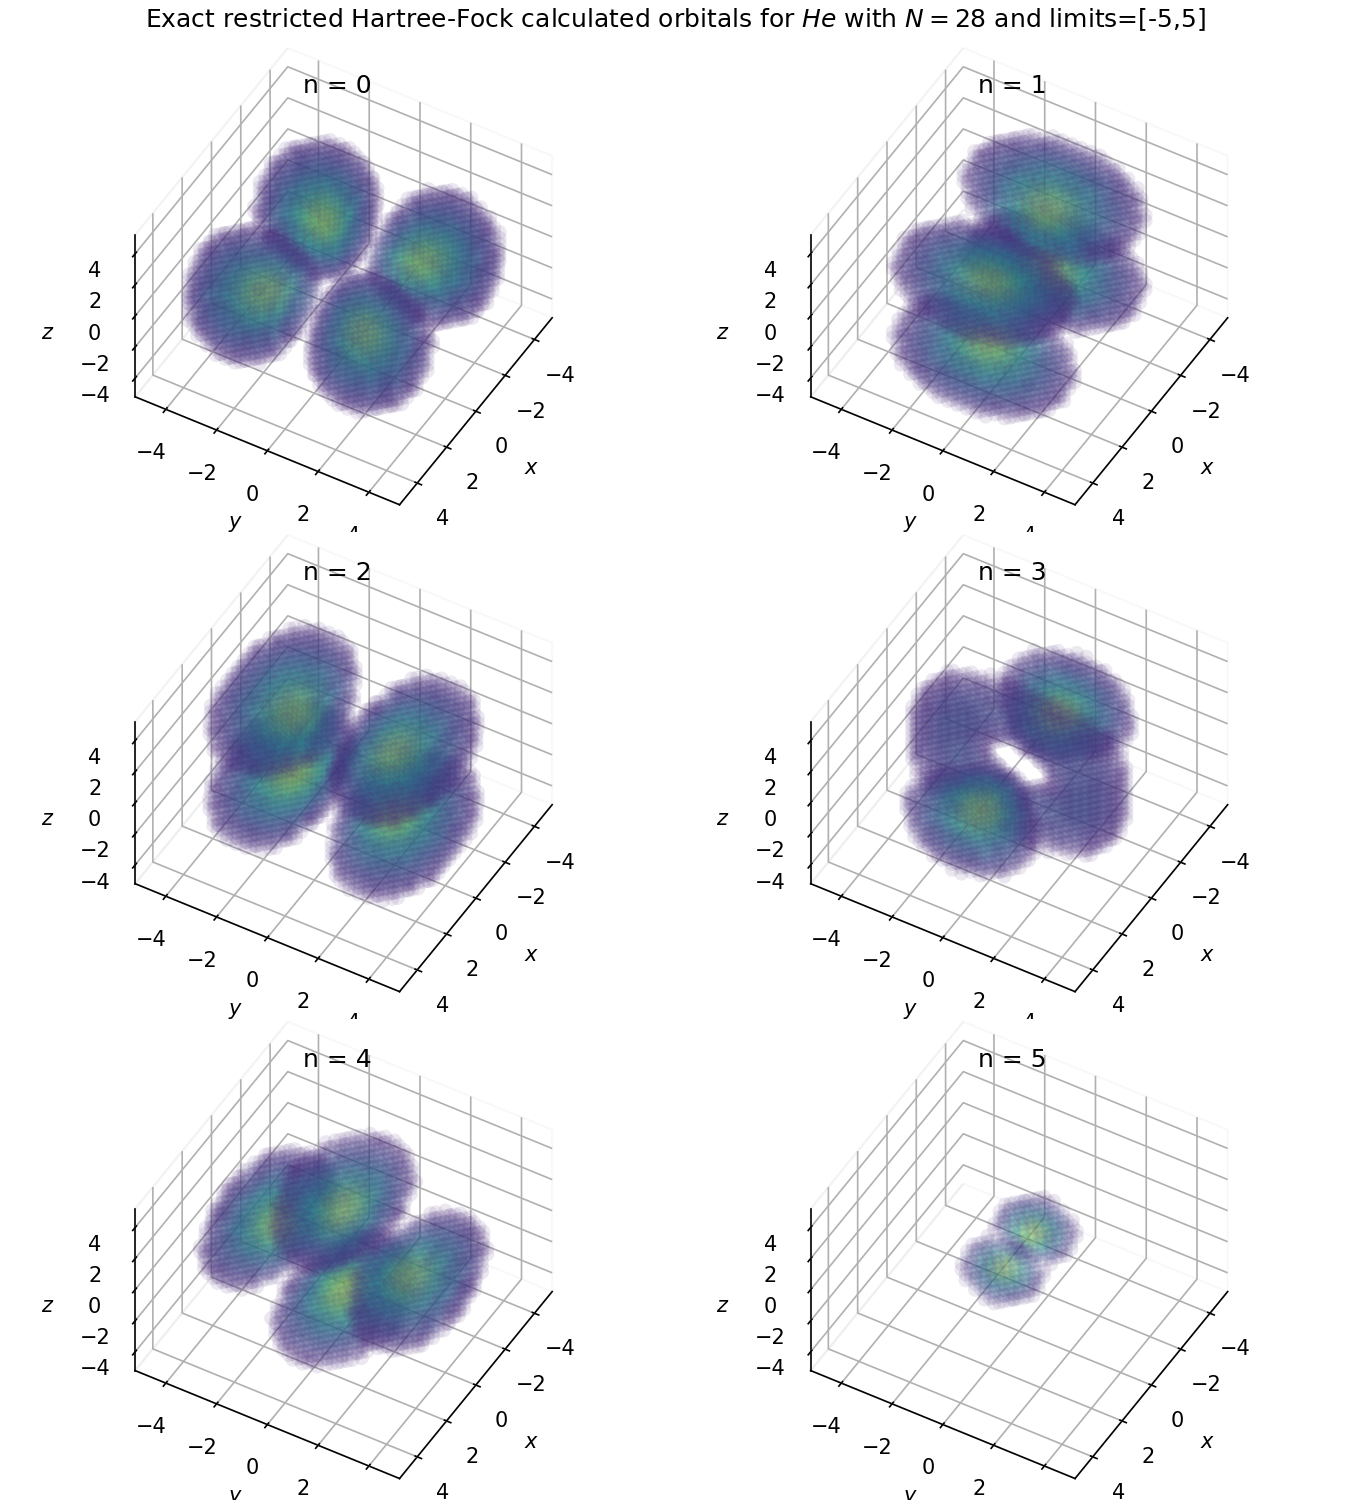
\includegraphics[scale=0.75]{he_N28_l5.png}
  \end{center}
  \caption{Calculated orbitals for $He$ atom using limits of [-5,5]}
  \label{he-plot}
\end{figure}

\begin{table}[H]
\begin{center}
\begin{tabular}{l|llllll}\hline
$n$    & $1$    & $2$     & $3$     & $4$      & $5$      & $6$      \\\hline
$E_n$  & $-0.049968$  & $-0.049878$  & $-0.041970$  & $0.011558$  & $-0.007816$  & $0.065703$ \\\hline
\end{tabular}
\end{center}
  \caption{The first six orbital energy levels obtained from applying HF to the Helium atom using limits of [-5,5]}
  \label{orbital-energies-he}
\end{table}

\newpage
\section{Discussion}

\begin{itemize}
    \item 
\end{itemize}

\newpage
\section{Code Listings and Data}

\subsection{Python Code Listing}
\label{code-listing-python}
The following is the code written in Python to generate the solutions and plots used in this report.
\lstinputlisting[language=Python]{basis-hartree-fock-sim.py}

\nocite{*}

\newpage
\bibliographystyle{IEEEtran}
\bibliography{IEEEabrv, refs}

\end{document}

